\subsection{Generacion de la nueva instancia} 
Para esta parte de la experimentaci�n, creamos nuevas instancias con el generador aleatorio y corrimos la misma instancia con las tres
heur�sticas,
para comparar las soluciones obtenidas y el tiempo de invertido en obtenerlas.

\subsection{Comparaci�n temporal}

A continuaci�n presentamos la comparaci�n temporal entre gr�ficos de distintas densidades. 
L�ase densidad para grafos, como el porcentaje de aristas con respecto al total posible de aristas ($n^2$, con n la cantidad de nodos). 

Respectivamente, los gr�ficos representan las comparaciones para gr�ficos con un 50 $\textperthousand$, 75 $\textperthousand$ y 
100 $\textperthousand$ de aristas. Podemos ver que la relaci�n entre todas se mantiene equivalente.



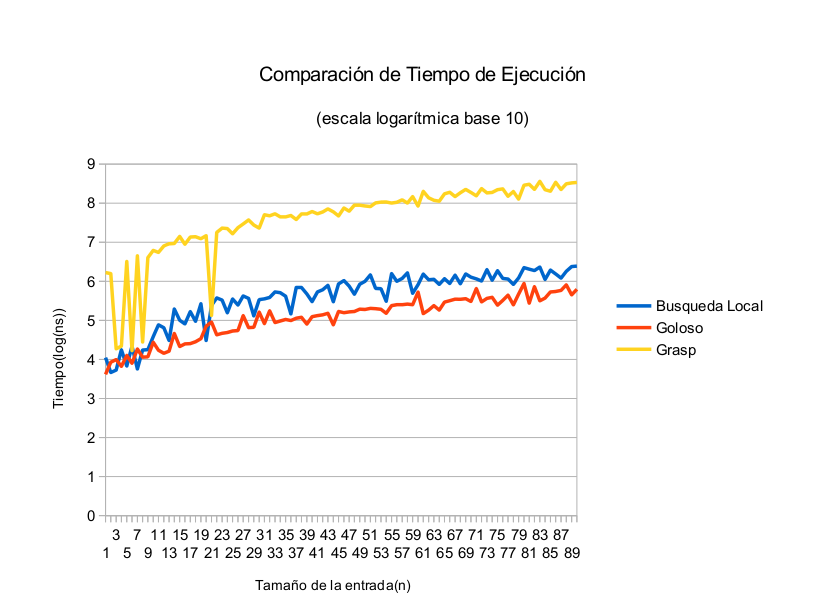
\includegraphics[width=1\textwidth]{heuristicas_grafico_densidad_50.png}

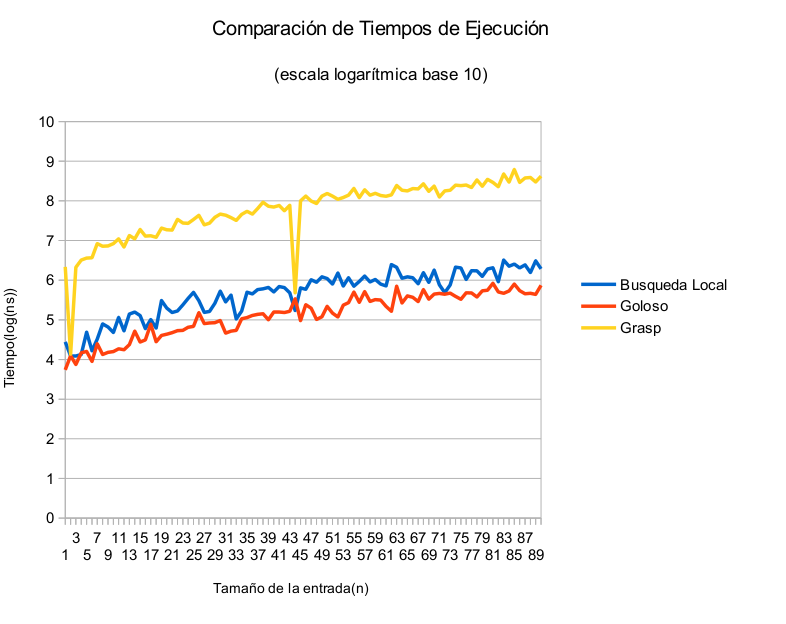
\includegraphics[width=1\textwidth]{heuristicas_grafico_densidad_75.png}

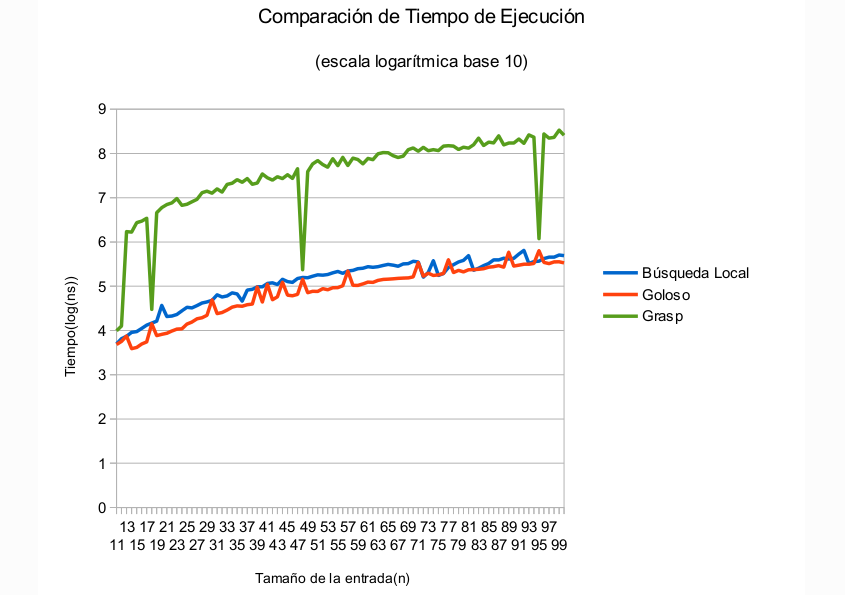
\includegraphics[width=1\textwidth]{heuristicas_grafico_densidad_100.png}



\subsection{Comparaci�n funcional} Comparaci�n entre las respuesta obtenidas.
A continuaci�n presentamos un gr�fico que detalla la diferencia entre los caminos m�nimos obtenidos por cada heur�stica. Como era de 
esperar, la heur�stica Grasp devuelve los caminos de menor peso en la mayor�a de los casos. 

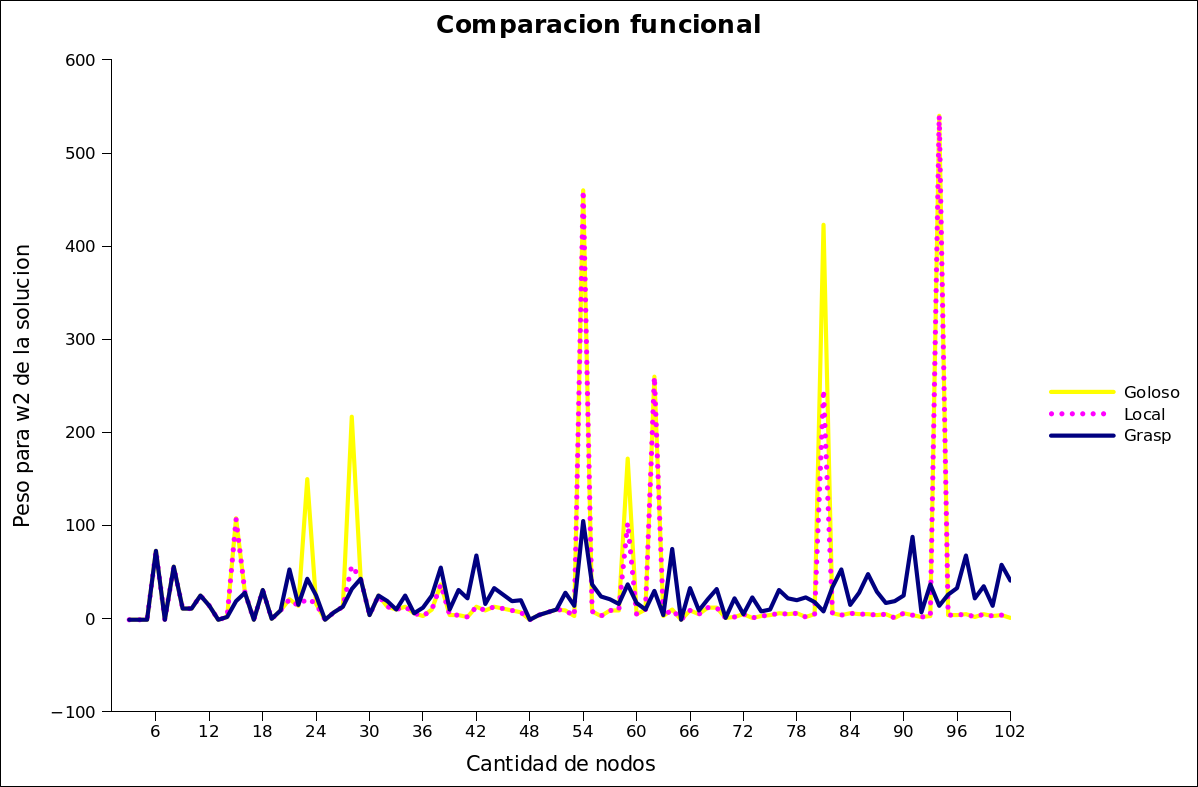
\includegraphics[width=0.8\textwidth]{compFunc}



\subsection{Comparaci�n con la soluci�n �ptima}
A continuaci�n presentamos una tabla que detalla la diferencia entre los caminos m�nimos obtenidos por cada heur�stica comparados con el 
algoritmo exacto. como se puede observar, excepto en las filas con $\sharp$Vertices 9, 13 y 15, las heur�sticas devuelven un resultado 
id�ntico al generado por el algoritmo exacto, esto se debe a que todav�a los grafos son peque�os y es mas probable que las heur�sticas 
encuentren el camino exacto. en las filas con $\sharp$Vertices 9, 13 y 15 es notable la diferencia entre resultados de las heur�sticas, 
dando grasp una soluci�n mucho mejor que las otras dos.
\begin{center}
  \begin{tabular}{| l | c | r | c | r | c | r | c | r | c | r | }
    \hline
	$\sharp$Vertices & $\sharp$Aristas & W2 Exacto & W2 Local & W2 Goloso & W2 Grasp\\ \hline
	1 & 0 & no & no & no & no  \\ \hline
	2 & 1 & 40 & 40 & 40 & 40 \\ \hline
     	3 & 3 & no & no & no & no \\ \hline
	4 & 6 & 25 & 25 & 25 & 25 \\ \hline
	5 & 10 & 54 & 54 & 54 & 54 \\ \hline
	6 & 15 & no & no & no & no \\ \hline
	7 & 21 & 8 & 8 & 8 & 8 \\ \hline
	8 & 28 & no & no & no & no \\ \hline
	9 & 36 & 71 & 238 & 238 & 71 \\ \hline
	10 & 45 & 28 & 28 & 28 & 28 \\ \hline
	11 & 55 & 29 & 29 & 29 & 29 \\ \hline
	12 & 66 & 10 & 10 & 10 & 10 \\ \hline
	13 & 78 & 38 & 111 & 167 & 38 \\ \hline
	14 & 91 & 38 & 38 & 38 & 38 \\ \hline
	15 & 105 & 43 & 107 & 209 & 43 \\ \hline


     \hline
   \end{tabular}
 \end{center}
 

